% ****** Start of file apssamp.tex ******
%
%   This file is part of the APS files in the REVTeX 4.1 distribution.
%   Version 4.1r of REVTeX, August 2010
%
%   Copyright (c) 2009, 2010 The American Physical Society.
%
%   See the REVTeX 4 README file for restrictions and more information.
%
% TeX'ing this file requires that you have AMS-LaTeX 2.0 installed
% as well as the rest of the prerequisites for REVTeX 4.1
%
% See the REVTeX 4 README file
% It also requires running BibTeX. The commands are as follows:
%
%  1)  latex apssamp.tex
%  2)  bibtex apssamp
%  3)  latex apssamp.tex
%  4)  latex apssamp.tex
%
\documentclass[%
reprint,
superscriptaddress,
citeautoscript,
%groupedaddress,
%unsortedaddress,
%runinaddress,
%frontmatterverbose, 
%preprint,
%showpacs,preprintnumbers,
%nofootinbib,
%nobibnotes,
%bibnotes,
 amsmath,amssymb,
 aps,
 prl,
%pra,
%prb,
%rmp,
%prstab,
%prstper,
floatfix,
]{revtex4-1}

\usepackage{graphicx}% Include figure files
\usepackage{dcolumn}% Align table columns on decimal point
\usepackage{bm}% bold math
\usepackage{color,soul} % highlight text
\usepackage{subfigure} % add by zigeng
%\usepackage{hyperref}% add hypertext capabilities
%\usepackage[mathlines]{lineno}% Enable numbering of text and display math
%\linenumbers\relax % Commence numbering lines

%\usepackage[showframe,%Uncomment any one of the following lines to test 
%%scale=0.7, marginratio={1:1, 2:3}, ignoreall,% default settings
%%text={7in,10in},centering,
%%margin=1.5in,
%%total={6.5in,8.75in}, top=1.2in, left=0.9in, includefoot,
%%height=10in,a5paper,hmargin={3cm,0.8in},
%]{geometry}

\begin{document}


\preprint{APS/123-QED}

% \title{Predicting band gap correction for perovskite oxide using high throughput and machine learning}
% \title{Accurate Prediction of Perovskite Oxides Band Gaps}
\title{Correcting band gaps and band-edge positions of oxide perovskites \\using DFT and  machine learning}

% Force line breaks with \\
%\thanks{A footnote to the article title}%

\author{Wei Li}
\thanks{These authors contributed equally to this work.}
\affiliation{Department of Materials Science and Engineering, University of Delaware, Newark, DE 19716, USA}
\author{Zigeng Wang}
\thanks{These authors contributed equally to this work.}
\affiliation{Computer Science and Engineering Department, University of Connecticut, CT 06269, USA}
\author{Xia Xiao}
\affiliation{Computer Science and Engineering Department, University of Connecticut, CT 06269, USA}
\author{Zhiqiang Zhang}
\affiliation{Department of Physics, University of Delaware, Newark, DE 19716, USA}
\author{Anderson Janotti}
\email{janotti@udel.edu}
\affiliation{Department of Materials Science and Engineering, University of Delaware, Newark, DE 19716, USA}
\author{Rajasekaran Sanguthevar}
\affiliation{Computer Science and Engineering Department, University of Connecticut, CT 06269, USA}
\author{Bharat Medasani}
\email{mbkumar@gmail.com}
\email{bmedasan@pppl.gov}
\affiliation{Delaware Energy Institute, University of Delaware, Newark, DE 19702, USA}
\affiliation{Princeton Plasma Physics Laboratory, Princeton, NJ 08540}



\date{\today}% It is always \today, today,
             %  but any date may be explicitly specified
\begin{abstract}

Density functional theory within the local or semilocal density approximations (DFT-LDA/GGA) has become a workhorse in electronic structure theory of solids, being extremely fast and reliable for energetics and structural properties, yet remaining highly inaccurate for predicting band gaps of semiconductors and insulators. Accurate prediction of band gaps using first-principles methods is time consuming, requiring hybrid functionals, quasi-particle GW, or quantum Monte Carlo methods.  Efficiently correcting DFT-LDA/GGA band gaps and understanding the main chemical and structural factors involved in the band-gap correction is desirable for discovering novel materials in high-throughput calculations.  In this direction, we use DFT and machine learning techniques to correct  band gaps and band-edge positions of semiconductors, using a representative subset of ABO$_3$ perovskite oxides as example. Relying on results of HSE06 hybrid functional calculations as target values of band gaps, we find a systematic band gap correction of $\sim$1.5 eV for this class of materials, where $\sim$1 eV comes from downward shifting the valence band and $\sim$0.5 eV from uplifting the conduction band. The main chemical and structural factors determining the band gap correction are determined through the feature selection procedure. 

%\begin{description}
%\item[Key words]
%Secondary publications and information retrieval purposes.
%\end{description}
\end{abstract}

%\pacs{Valid PACS appear here}% PACS, the Physics and Astronomy
                             % Classification Scheme.
%\keywords{Suggested keywords}%Use showkeys class option if keyword
                              %display desired
\maketitle

%\tableofcontents

\section{Introduction}
 
 \begin{figure}[ht]
\begin{center}
\includegraphics[width=3.0 in]{Figures/Fig1_v1.eps}
\end{center}
\caption{Crystal structures of ABO$_3$ perovskite prototypes. Green, blue and red spheres represent of A, B and O atoms, respectively.  crystal structure of (a) $Pm\bar{3}m$ cubic structure, (b) $I4_mmm$ tetragonal structure, (c)  $Pnma$ orthohombic structure and (d) $R\bar{3}c$ Rhombohedral. The apical and equatorials B-O-B bond angles, $\alpha_{a}$ and $\alpha_{e}$ are indicated in (e). The A and B atoms selected for this study are indicated in the Periodic Table in the lower panel.
}
\label{fig1}
\end{figure}

The band gap and band-edge positions (i.e., ionization energy and electron affinity) are basic properties of semiconductors and insulators, and often dictate applications. Their prediction, based on first-principles methods, play central role in novel materials discovery. DFT calculations \cite{Kohn1964,Kohn1965} based on LDA\cite{Hohenberg1964} or GGA\cite{Perdew1996} are often used to predict stable crystal structures, with lattice parameters within 1-2\% of the experimental values\cite{Tran2016,Lianhua2014}. These calculations are extremely fast and scalable, permitting the study of the energetic and structural properties of thousands of materials with relatively modest computing resources and in relatively short times, playing a key role in current materials discovery research efforts based on high-throughput computation. However, band gaps ($E_g$) are severely underestimated compared with the experimental values when standard LDA or GGA functionals are employed. Predicting $E_g$ of semiconductors and insulators requires going beyond LDA or GGA approximations in DFT, making the calculations much more involved and computationally expensive.

Methods that accurately predict band gaps are computationally expensive regarding both computational resources and timing. The simplest approach is to mix Fock exchange with GGA exchange in a hybrid functional \cite{Becke1993,Perdew1996_1,Heyd2003,Heyd2006}, partially correcting the self-interaction error in DFT-LDA/GGA, giving band gaps very close to the experimental values for many materials\cite{Brothers2008,Xiao2011,Kim2009,Henderson2011}. This increases the computation time by ten fold compared to DFT-LDA/GGA calculations. More formally rigorous approaches would be to use the Green’s function quasi-particle GW \cite{Luoie1996,Kresse2006,Chen2015} or the wavefunction-based quantum Monte Carlo\cite{Hunt2018,Yang2020,Hunt2020} method, yet at the expense of at least an extra order of magnitude in computational time. As a result, these are not generally amenable to high-throughput computational approaches, posing obstacles to novel materials discovery. 

Machine learning (ML) techniques have emerged as powerful tools in materials science research, with applications in a variety of directions, such as prediction and classification of crystal structures \cite{Fischer2006,CARR2009339,Pilania2015,Yamashita2018,Ye2018}
% development of interatomic potentials \cite{Hobday1999,Handley2010,Schneider2017}, 
and building predictive models of  various materials properties \cite{Pilania2013,Lee2016,Pilania2016,Bart2017}, 
% even finding optimal functionals for density functional theory \cite{Wellendorff2012,Snyder2012,Brockherde2017,Pilania2013}. 
Recent efforts also include predicting band gaps, however with limited accuracy \cite{Zhuo2018,Lu2018,Xie2018,Allam2018,Olsthoorn2019}. A straightforward direction would be to predict band gaps using the DFT-GGA band structures available in AFLOW database \cite{Curtarolo2012} as a training set for machine learning approaches. However, this would have limited use considering that the predicted band gaps would still be severely underestimated. Or one could use DFT+U \cite{Anisimov1997} for band gaps, with computational costs similar to those of DFT-LDA/GGA; the problem is be what value of $U$ to choose and the justification of applying $U$ to dispersive valence and conduction bands. An interesting approach involves graph convolutional neural networks (CGCNN) based on atomic connections in the crystal structure after being trained using DFT band gaps \cite{Xie2018}. However, this method was also trained and aimed at DFT-GGA band gaps. Recently, reports on automated, high-throughput calculations of band gaps based on hybrid functional have appeared in the literature \cite{Weng2019,Jie2019,Pilania2017,Ward2016,Huang2019}, pointing toward more reliable predictions of band gaps, yet the nature and size of the band-gap corrections from the DFT-GGA values have not been discussed or analyzed.

\begin{figure*}[ht]
\begin{center}
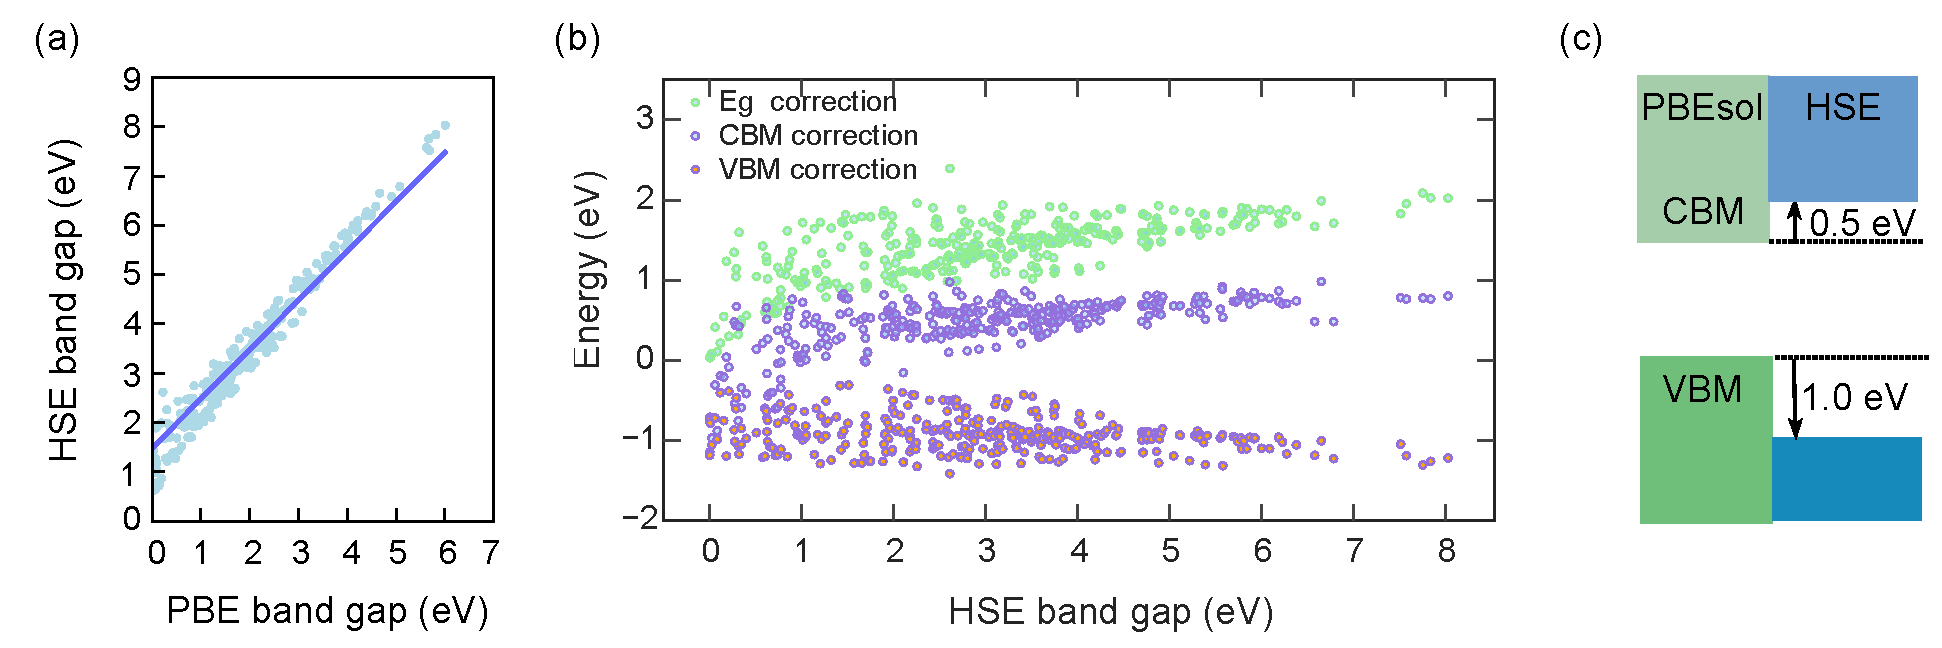
\includegraphics[width=6in]{Figures/fig2.eps}
\end{center}
\caption{Correction of the band gap of ABO$_{3}$ perovskites based on HSE06 and DFT-GGA PBEsol calculations. (a) HSE06 vs PBEsol band gaps, (b) the band-gap correction ($\Delta E_{g}$, light green), the correction of the valence-band maximum $\Delta{\rm VBM}$ (light blue) and conduction-band minimum $\Delta{\rm CBM}$
(dark red) vs HSE06 band gap. (c) schematic of the correction of the band-edge of the positions. The line in (a), placed to guide the eye, represents a regression with slope equal 1 and crosses the vertical axis at 1.5 eV. 
}
\label{fig2}
\end{figure*}

In this work we developed machine learning models for mapping band gaps computed with DFT-GGA into band gaps as calculated using the HSE06 hybrid functional. We choose perovskite oxides as example to demonstrate the applicability of our approach, making the case that HSE06 predicts accurate band gaps for a representative subset of this class of materials. An interesting feature of ABO$_{3}$ perovskite semiconductors and insulators is the dependence of their band  gaps on the metal elements A and B as well as on rotations and tilting of the BO$_6$ octahedra. Here we restrict the scope of perovskite materials to those for which the valence band is derived from oxygen 2$p$ orbitals and the conduction band is derived from A or B valence orbitals, as indicated in Fig.~\ref{fig1}. I.e., we did not consider perovskites where the valence and conduction bands are determined by transition metal $d$ orbitals and the gap associated with $d$-$d$ transitions. We also include octahedral tilting and rotations leading to tetragonal, orthorhombic, and rhombohedral crystal structures as shown in Fig.~\ref{fig1}. Basically, we calculated $E_{g}$ with DFT-GGA and HSE06 via a high-throughput approach and employed different machine learning models to predict the HSE06 band gaps, by which we analyze the corrections to the valence-band maximum (VBM) and conduction-band minimum (CBM) separately. Our combined DFT-ML model predicts $E_{g}$ within an error of 0.16 eV, and reveals the main atomic and structural factors that determine the correction of the VBM, CBM, and consequently $E_{g}$. 

\section{Methods and computational details}

Our first-principles calculations are based on DFT within the generalized gradient approximation of Perdew, Burke, and Ernzerhof revised for solids (PBEsol)  \cite{Perdew} and the projector augmented wave  method \cite{Blochl1994,Kresse1999} as implemented in the Vienna Ab initio Simulation Packaged (\textsc{VASP}) \cite{Kresse1993a,Kresse1993b}.
The wave functions are expanded in plane waves with cutoff energy of 650 eV. Structure optimizations are performed using 7$\times$7$\times$7, 7$\times$5$\times$7, 7$\times$5$\times$5, and 7$\times$7$\times$7 $\Gamma$-centered $k$-point grid for the integrations over the Brillouin zones of the cubic, tetragonal, orthorhombic, and rhombohedral primitive cells, respectively. The screened hybrid functional  HSE06  \cite{Heyd2003,Heyd2006} is employed to compute target band gaps, using the structural parameters found using the PBEsol functional. In tests we find that PBEsol and HSE06 give lattice parameters that differ by less than 1\%, and in good agreement with experimental values. So we neglected the differences in the band gap calculated using the PBEsol-optimized lattice parameters and those calculated using the HSE06-optimized lattice parameters. Test calculations indicate that these differences are less than 0.1 eV.
 

We used different ML algorithms to build our band-gap prediction model, including the linear ridge regressor (LRR), kernel ridge regressor (KRR), and gradient boosted decision tree (GBDT) from open-source software package Scikit-Learn Toolbox~\cite{scikit-learn}.  
To set the hyperparameters in the models, we used 3-fold cross-validated scheme for hyperparameters tuning by grid search and creating the training and test data sets.
The input to the model is comprised of atomic and structural properties, including
the B-O-B apical angle $\alpha_{a}$ and B-O-B equatorial angle $\alpha_{e}$.
The regression fit to the input gives the predicted band gaps. Prediction performance of the learning models is evaluated by the mean-absolute error (MAE). 
The feature importance of all the descriptors is obtained with GBDT to interpret the importance of various descriptors in the training model.

\section{Results and Discussions}

We selected 118 oxide perovskites ABO$_{3}$, and for each we considered four crystal structures, with symmetries $Pm\bar{3}m$ (cubic), $I4_mmm$ (tetragonal), $Pnma$ (orthorhombic) and $P63/mmc$ (rhombohedral), as shown in Fig.~\ref{fig1}, totaling 472 structures. The selected A and B atoms, also indicated in the Periodic Table in Fig.~\ref{fig1}, are: A = Li, Na, K, Rb, Cs, Cu, Ag, Au, Be, Mg, Ca, Sr, Ba, Pb, Zn, Cd, Sn, Sc,Y, La, or Bi, and B = P, As, Sb, V,  Nb, Ta, Si, Ge, Sn, Ti, Zr, Hf, Al, Ga, In, or Tl, such that the considered compounds satisfy valence(A)+valence(B)=6. A data set of DFT-GGA band gaps was constructed using this set of materials.

\begin{figure*}[ht]
\begin{center}
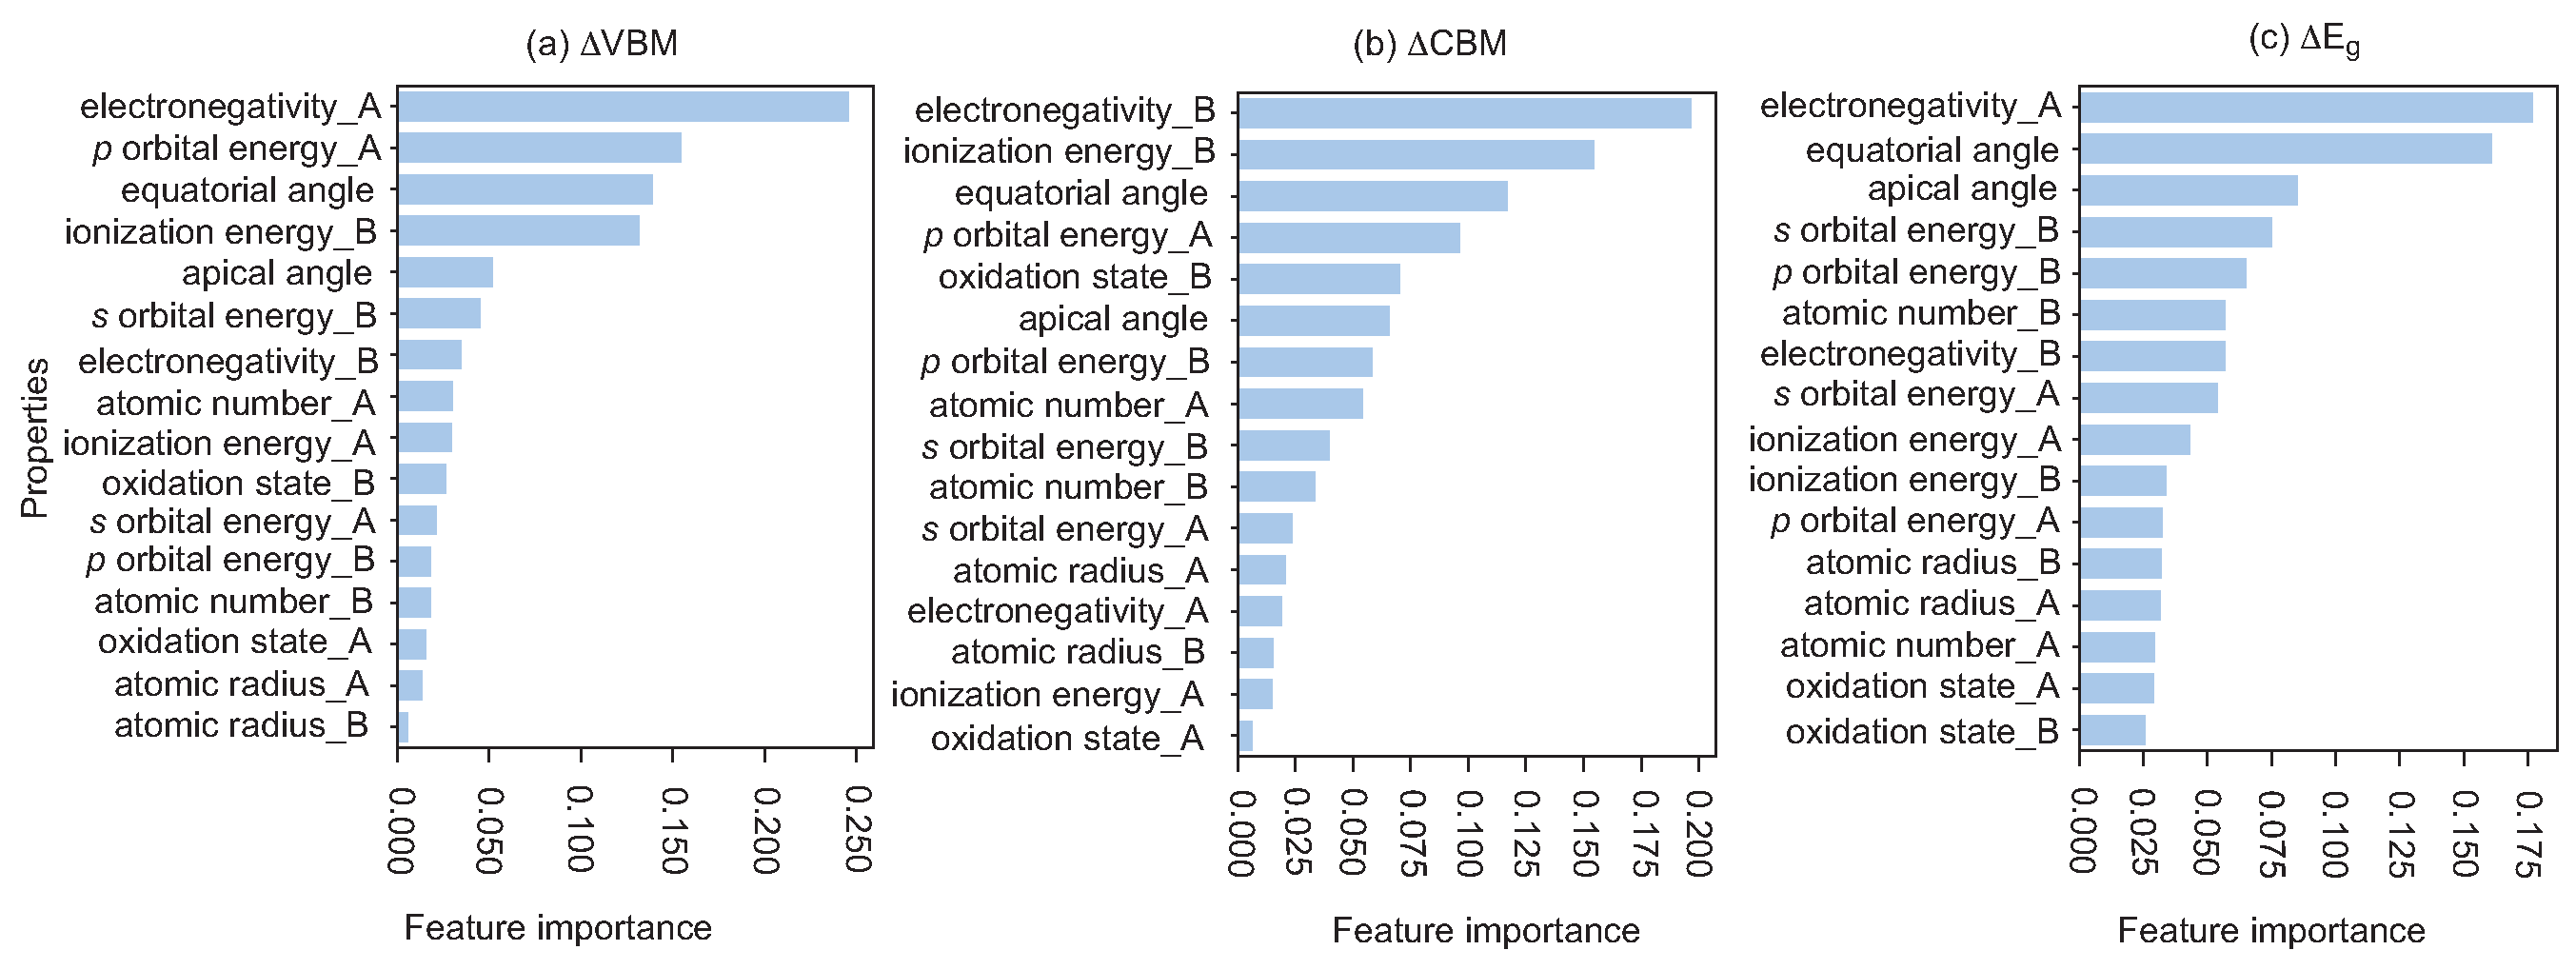
\includegraphics[width=6.6in]{Figures/feature_ranking_gap.eps}
\end{center}
\caption{Feature importance in the gradient boosted decision tree (GBDT) model for determining the band-gap ($\Delta E_{g}$) and band-edge corrections ($\Delta {\rm VBM}$, $\Delta {\rm CBM}$) of ABO$_3$ perovskites. 
}
\label{fig3}
\end{figure*}

The four crystal structures for all ABO$_{3}$ compounds were first optimized with the DFT-GGA PBEsol functional. Then their electronic structures were calculated using PBEsol and HSE06. In this way, since the average electrostatic potential is used as reference for the Kohn-Sham band energies, and does not depend on exchange and correlation, we can directly compare the PBEsol and HSE06 band structures, extracting the corrections for VBM and CBM, and the band gap (i.e., $\Delta {\rm VBM}$, $\Delta {\rm CBM}$, and $\Delta E_{g}$).  We note that for all compounds studied, the VBM for the cubic structure occurs at the R point (0.5, 0.5, 0.5) and the CBM occurs at the $\Gamma$ point in the cubic Brillouin zone, characterizing an indirect R-$\Gamma$ fundamental band gap.  For the tetragonal, orthorhombic, and rhombohedral structures, both VBM and CBM occur at $\Gamma$, characterizing a direct $\Gamma$-$\Gamma$ fundamental band gap. 

The calculated HSE06 band gap vs PBEsol band gap are shown in Fig.~\ref{fig1}(a). First, we note that the DFT-GGA underestimates the band gap with respect to HSE06 by $\sim$1.5 eV. The largest deviation from this trend are observed for compounds containing Cu, Pb, and Sn occupying the A site. In the case of Cu-B-O$_3$ compounds, the Cu $d$ orbitals mix with the O 2$p$ orbitals, pushing the VBM to higher energies. In the case of Sn-B-O$_3$ and Pb-B-O$_3$, the VBM has large contributions from Sn and Pb $s$ valence orbitals, which also pushes the VBM to higher energies. In all the cases where the valence band is mostly derived from O 2$p$ orbitals, the $\sim$1.5 eV band-gap correction fits the data quite well.  
We also note that the HSE06 band gaps are in good agreement with available experimental data as listed in the Table I in the supplemental material, justifying our use of HSE06 as target experimental values for band gaps.

The separated corrections $\Delta {\rm VBM}$ and $\Delta {\rm CBM}$, i.e., the amount the VBM and CBM in HSE06 differ from the VBM and CBM in DFT-GGA are shown in Fig.~\ref{fig2}(b). Contrary to common wisdom, where it is often assumed that to correct the DFT-GGA band gap only an upward shift of the CBM is necessary, we find that about 2/3 of the gap correction comes from shifting down the VBM and only about 1/3 of the correction comes from shifting the conduction band upward. This can be attribute to large self-interaction correction of the O 2$p$ derived valence bands in these materials.  Again, the outliers, where the VBM is corrected by a lesser amount, correspond to compounds containing Cu, Sn, or Pb in the A site. It is also interesting to note the correction in the VBM derived from O 2$p$ is larger than the correction of CBM derived from $d$ orbitals, such as in SrTiO$_3$ and similar compounds, despite the rather flat nature of their conduction bands that are derived from the quite localized transition metal $d$ orbitals. Finally, we also note that the band-gap correction $\Delta E_{g}$ is slightly larger than 1.5 eV for compounds with larger band gaps, approaching 2 eV, and this is traced back to the correction of the CBM which approached 1 eV for compounds with $E_g$ $\gtrsim$ 4 eV.

Having established the band-gap correction for these oxide perovskites, we now turn to machine learning techniques to develop a model that correlates the $\Delta {\rm VBM}$, $\Delta {\rm CBM}$, and $\Delta E_{g}$ corrections to atomic and structural properties of the compounds. The list of atomic properties include electronegativity, ionization energy, valence-orbital energies, and atomic radius of both A and B atoms. Structural properties include octahedral tilting and rotations that are characterized by the apical $\alpha_{a}$ and equatorial $\alpha_{e}$ angles corresponding to B-O-B angles parallel and perpendicular to the $c$ axis. We employed three machine learning models, which are the linear ridge regressor (LRR), kernel ridge regressor (KRR), and the gradient boosted decision tree (GBDT) classifiers,
as implemented in Scikit-Learn Toolbox~\cite{scikit-learn}. We used a regularization strength of $0.01$ to both LRR and KRR models. We have used polynomial kernel in KRR with maximum order $3$. For the GBDT model, we set the maximum tree depth to $5$ with $500$ base estimators.

\begin{table}[htbp]
  \centering
  \caption{Mean absolute error (MAE) used to evaluate the performance of the linear ridge regressor (LRR), kernel ridge regressor (KRR), and the gradient boosted decision tree (GBDT) models in predicting the corrections of the valence-band maximum ($\Delta {\rm VBM}$), conduction-band minimum ($\Delta {\rm CBM}$) and band gap ($\Delta E_{g}$) of oxide perovskites in DFT-GGA PBEsol compared to the HSE06 values. }
    \begin{tabular}{llll}
    \hline\hline
          & \ \ \ \ \ LRR   & \ \ \ \ \ KRR   & \ \ \ \ GBDT \\
    \hline
    $\Delta {\rm VBM}$ \  \ & $0.10 \pm 0.01$ \ \ & $0.09 \pm 0.01$ \ \ & $0.09 \pm 0.01$ \\
    $\Delta {\rm CBM}$ \ \ & $0.19 \pm 0.01$ \  \ & $0.15 \pm 0.01$ \ \ & $0.10 \pm 0.003$ \\
    $\Delta E_{g}$ \ \ & $0.23 \pm 0.02$ \ \ & $0.20 \pm 0.01$ \ \ & $0.16 \pm 0.01$ \\
    \hline
    \end{tabular}%
  \label{tab:comp}%
\end{table}%

%%%%%%%%%%
The prediction performance of the LRR, KRR, and GDBT models can be seen in 
Table.~\ref{tab:comp}. In these models we use 2/3 of the data as training set. We also use mean absolute error (MAE) to measure the performance in predicting $\Delta {\rm VBM}$, $\Delta {\rm CBM}$, and $\Delta E_{g}$. Among the three models, GBDT gives the highest prediction accuracy and the lowest variance; the KRR model performs better than LRR.  Note that we obtain lower MAE than previous models \cite{Zhuo2018,Gladkikh2020,Pilania2017,Zhuo2018,Rajan2018}, likely to the better quality or more uniformity of our training dataset. The results indicate that there exists a complex nonlinear relation between the input properties and the target results, explaining why the pure linear model LRR performs poorly.  Note that all the three ML models predict $\Delta {\rm VBM}$ with similar performance, indicating that the VBM correction has a more linear relation with the input properties than the CBM and $E_g$ corrections.

What are the main atomic and structural properties that determine the band-gap and band-edge corrections? The answer is shown in Fig.~\ref{fig3}, where the input properties that were used in the GDBT model are ranked according to their importance. We find that the electronegativity, the energy of $p$ valence orbital of atom A, and the equatorial angle of the octahedral rotation are the main properties that determine $\Delta {\rm VBM}$. For $\Delta {\rm CBM}$, the main properties are the electronegativity, ionization energy of atom B atom and the equatorial angle of the octahedral rotation.
  
For both $\Delta {\rm VBM}$ and $\Delta {\rm CBM}$, the equatorial angle determines the overlap between the orbitals of B and O in the directions parallel to the $a$-$b$ plane, which in turn, affect both VBM and CBM positions. Note that the dependence on the apical angle $\alpha_a$ is less than that on the equatorial angle $\alpha_e$ since the former affects the B-O orbital overlap only along the $c$ direction.  Finally, we also note that the relative importance of the electronigativity, ionization energies, and rotation angles is higher for atom A than for atom B in determining the band gap.  This is attributed to the larger contribution of the VBM correction than the CBM correction to $\Delta E_{g}$.


\section{Summary}

Using high-throughput DFT-GGA PBEsol and HSE06 calculations we determined the band gap correction of a representative set of oxide perovskites, finding that the HSE06-based correction pushes down valence band by $\sim$1 eV and pushes up conduction band by $\sim$0.5 eV. These results are then used in machine learning models that include atomic and structural properties as input to determine the corrections to the valence band, conduction band, and band gap. The properties used as fitting parameters are ranked according to their relative importance to the corrections. We find that electronegativity of the A and B atoms together with the equatorial angle of rotation of the BO$_6$ octahedra are the main factors involved in the corrections. These results serve as starting point and guide to developing novel machine-learning-based approaches applicable to the discovery of novel electronic materials.

\section{Data availability}

The datasets generated and/or analysed during the current study are available in
the GitHub repository https://github.com/....

\section{Acknowledgments}

This work was supported by the National Science Foundation Faculty Early Career Development Program DMR-1652994. This research was also supported by the the eXtreme Science and Engineering Discovery Environment (XSEDE) facility, National Science Foundation grant number ACI-1053575, and the Information Technologies (IT) resources at the University of Delaware, specifically the high performance computing resources. This research was also supported in part by the following National Science Foundation grants: 1447711, 1743418, and 1843025.

\bibliography{BIB}

\end{document}

% \begin{figure*}[ht!]
% \begin{center}
% 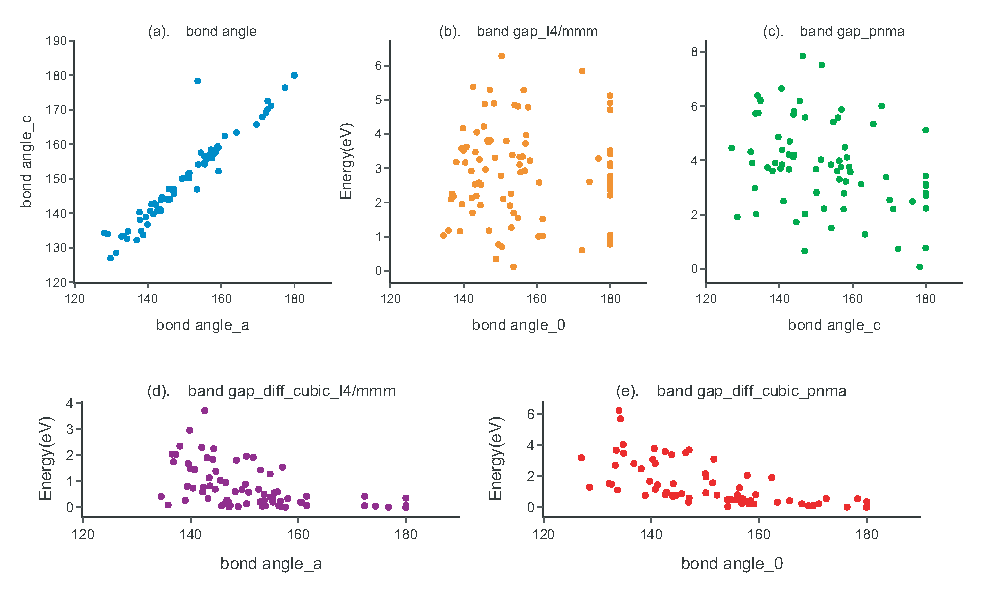
\includegraphics[width=6.0in]{Figures/Fig3.eps}
% \end{center}
% \caption{ (a) the correlation functional relationship between the equatorial and apical bond angle in the orthorhombic structure (space group $Pnma$).
% (b) The DFT band gap of the tetragonal structure (space group $I4_mmm$) as a function of the apical B-O-B bond angles. 
% (c) Two-dimensional map of the DFT band gap of the orthorhombic structure as a function of the apical B-O-B bond angles. 
% (e) The map of the DFT band gap difference between cubic structure and tetragonal structure. 
% (e) The map of the DFT band gap difference between cubic structure and orthorhombic structure. 
% }
% \label{fig4}
% \end{figure*}

% Fig 3. (a) is the map between the apical bond angle and equatorial bond angle in the $Pnma$ structure. It shows a linear function with apical bond angle $\approx$ equatorial bond angle, which is a correction() for the ref\cite{} investigation. 

% Based on our Fig 3.(b) and (c), there is no specific correlation between the DFT band gap and the B-O-B bond angle in the structure. We shows singnificant scatter data dispersion at all the range of the B-O-B bond angle when we change the AB combination. 

% One interesting comparison is the band gap relationship between the cubic (pm$3_bar$m) structure and tetragonal($I4mmm$)\& orthombhedral$pnma$ structure. With octahedral rotation, the band gap not surprisingly increase but always less than 1 eV as shown in Fig3 (d) and (e).


To be deleted:

% The band gap and band-edge positions (i.e., ionization energy and electron affinity) are basic properties of semiconductors, and often dictate applications. 
% Methods used to accurately predict band gaps are computationally expensive, in resources and timing. First-principles calculations based of the density functional theory (DFT)  are routinely employed to predict the most stable crystal structures, with lattice parameters within 1-2\% of the experimental values.
% these calculations are extremely fast and scalable, allowing for predictions of the energetics and structural properties of thousands of materials with relatively modest computing resources in relatively short times, playing a key role in current materials discovery research programs. 
% Predicting band gaps ($E_g$) of semiconductors and insulators requires going beyond the local or the generalized density approximations (LDA/GGA) in DFT, making the calculations much more involved and computationally expensive. The simplest approach is to mix Fock exchange with GGA exchange in a hybrid functional, partially correcting the self-interaction error in DFT-LDA/GGA, giving band gaps very close to the experimental values for many materials. This increases the computation time by ten fold compared to DFT-LDA/GGA calculations. More rigorous approaches would be to use the Green’s function quasi-particle GW \cite{Luoie1996,Kresse2006} or the wavefunction-based quantum Monte Carlo methods, yet at the expensive of an extra order of magnitude in computational time. Being able to correct band gaps obtained using DFT-LDA/GGA in a fast way and with minimum resources would greatly add to the computational materials discovery effort. 
% However, these methods are not currently amenable to high-throughput computation due to their excessive computational cost.

%  However, there is a systematic under-estimation of the band gap, E$_g$, compared with the experimental values when employing standard exchange and correlation functionals such as the generalized gradient approximation as proposed by Perdew, Burke, and Ernzerhof (PBE) \cite{Perdew1996}.  Hybrid functionals  \cite{Heyd2003,Heyd2006} or the Green’s function quasi-particle GW methods \cite{Luoie1996,Kresse2006} improve accuracy, but are much more expensive computationally, precluding their systematic use in searching over thousands of compounds. To accelerate the discovery and development of new functional materials, it is desirable to have an automating and scalable computational approach that predicts accurate values for band gaps at the speed or faster than DFT-PBE calculations. 


% Perovskite materials have garnered much attention due to having ideal band gaps for capturing solar light, leading to the design of photovoltaic systems \cite{Pilania2013,Lee2012,Yin2015,Liu2013,Burschka2013,Lee2012,Green2014}. A tremendous amount of potential element combinations can be considered within perovskite structures, suggesting that there should still be hidden and undiscovered perovskite materials useful for solar light capturing. So far, the main data for perovskite formability can be found in a few articles that summarize the existing experimental data and prevalent databases. High throughput first principle calculations have become a foundation for the “materials
% by design” paradigm \cite{Anubhav2013, Draxl2019,Montoya2017,Carrete2014,Tabor2018,Bassman2018,Dagdelen2017,Saal2013} and have previously been used to screen for potential perovskite materials for solar light capturing \cite{Huo2018, Sun2015}, but such calculations are found to leave unexplored spaces of perovskite materials due to the limitation of heavy computational times of the band gaps.

% Thus, trends and periodicities hidden within the data of 19000 perovskite materials are sought after and hidden perovskite materials for applications in capturing solar light are explored through the use of materials informatics.
% Several research groups have demonstrated the benefits of automating and scaling computational property. For example, an overview of high-throughput band structure calculations by Curtarolo et al. [6] New materials for radiation detectors is suggested by screening about 22,000 materials by Hachmann, et al. [7]

% Perovskite materials have garnered much attention due to having ideal band gaps for capturing solar light, leading to the design of photovoltaic systems 9−12 A tremendous amount of potential element combinations can be considered within perovskite structures, suggesting that there should still be hidden and undiscovered perovskite materials useful for solar light capturing.

% Machine learning has been recently used for novel perovskite designs owing to the availability of a large amount of applications because of the structure flexibility with multiple A-B-X combination. A tremendous amount of potential element combinations can be considered within perovskite structures, suggesting that there should still be hidden and undiscovered perovskite materials useful for solar light capturing. However, trustworthy results should be based on the valid and reliable data that can reveal the nature of materials as much as possible. We carefully generated the HSE and PBEsol datasets and it indicate that the valence band maximum (VBM) decreased 1 eV and conduction band minimum (CBM) increased 0.5 eV. We used machine learning with a multiple models approach accurately predict the HSE06 VBM, CBM and E$_{g}$ correction with accuracy of -0.145 eV, by quantitatively analyzing the valence band maximum (VBM) and conduction band minimum (CBM) offset. Not only does this resulting tool provide the ability to accurately predict the HSE06 band gap based on the PBEsol results but also the speed of the prediction based only on the cubic structure will make this a great resource to screen functional perovskite materials. And this design represents a powerful database and tool paves a way for mapping the vast materials landscape and accelerating discovery. 

%%%This could be included earlier....if we need to.
% The severe underestimation of band gaps in DFT-LDA/GGA stems from the discontinuity in the derivative of exchange and correlation potential as the number of electrons deviates from two subsequent integer occupations, associated with the self-interaction error in the Kohn-Sham orbital energies. Basically, DFT-LDA/GGA deviates from the expected straight-line behavior between two integer occupation numbers, following a convex curvature. This spurious self-interaction also leads to errors in electron localization, leading to more delocalized solutions. Hartree-Fock, on the contrary, shows a concave behavior for many-electron systems, resulting in localization of charges. A hybrid exchange and correlation function, which mixes a fraction of PBE with a fraction of Hartree-Fock, produces an almost straight-line behavior, as desired. The band gaps calculated using hybrid functionals show excellent agreement with the experimental results. However, the hybrid functional quantitative correction to the standard exchange and correction functional is still unknown and we are aiming to find a hidden trend of the band gaps.

%%%%%%
% Because both equatorial angle and apical angle determine the overlap of the B-O-B orbitals which is correlated with CBM, VBM, and band gap corrections, this intuitive picture is well captured by our model as shown in Fig.\ref{fig:feature_importance}. 

% The machine learning models help us in gaining a fundamental understanding of the most relevant features of the elements, such as atomic orbital energies, inter atomic distances, etc, in the determination of band gaps. We believe that this type of crude estimation of properties can be interesting supplements to standard features.  This crude estimation of properties consists of the calculation of a target property (the HSE06 functional band gap) utilizing crude estimators (the calculated PBEsol band gap). This machine learning algorithm no longer needs to predict a high cost target property but rather a correction or a difference between properties calculated with two well-defined methodologies.



% \begin{figure}[ht]
% \begin{center}
% 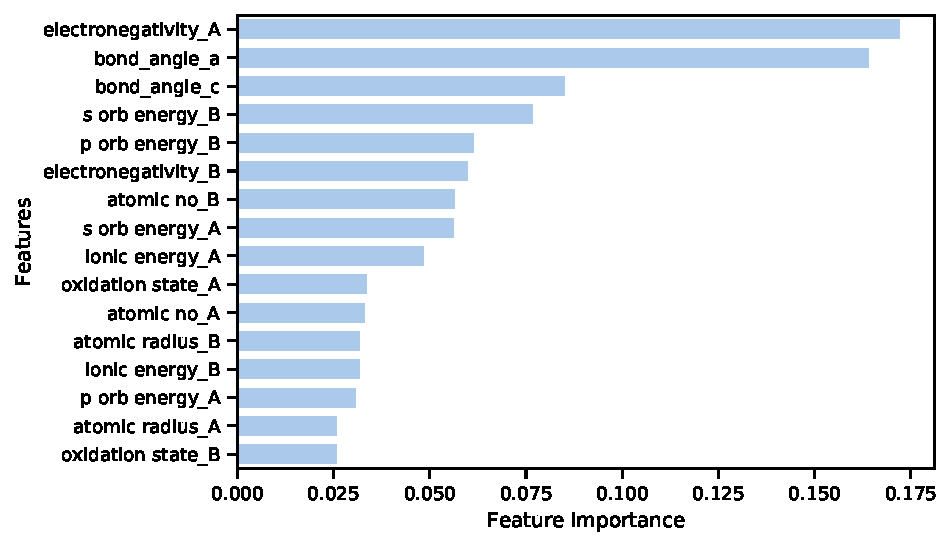
\includegraphics[width=3.4in]{Figures/feature_ranking.pdf}
% \end{center}
% \caption{Feature Importance Ranking}
% \label{fig3}
% \end{figure}

% \begin{figure}[htpb]%
% \centering
% \subfigure[Feature Ranking for CBM Prediction]{%
% \label{fig:cbm}%
% 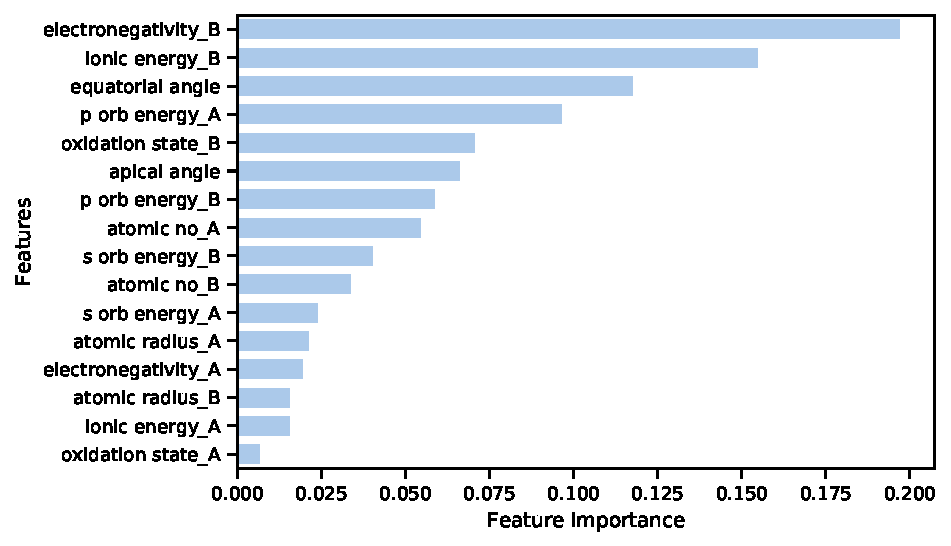
\includegraphics[width=3in]{Figures/feature_ranking_cbm.pdf}}%
% \\ 
% \subfigure [Feature Ranking for VBM Prediction]{%
% \label{fig:vbm}%
% 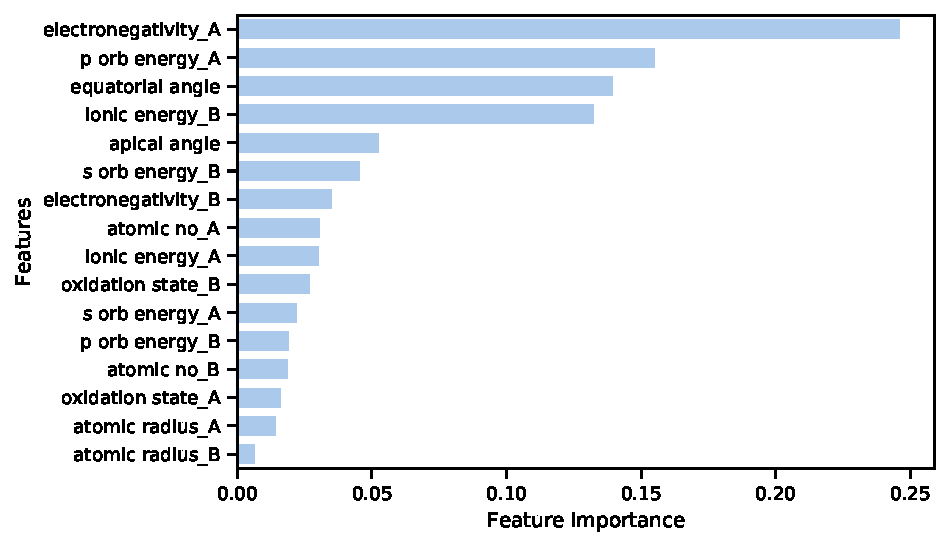
\includegraphics[width=3in]{Figures/feature_ranking_vbm.pdf}}%
% \\
% \subfigure [Feature Ranking for E$_{g}$ Prediction]{%
% \label{fig:bandgap}%
% 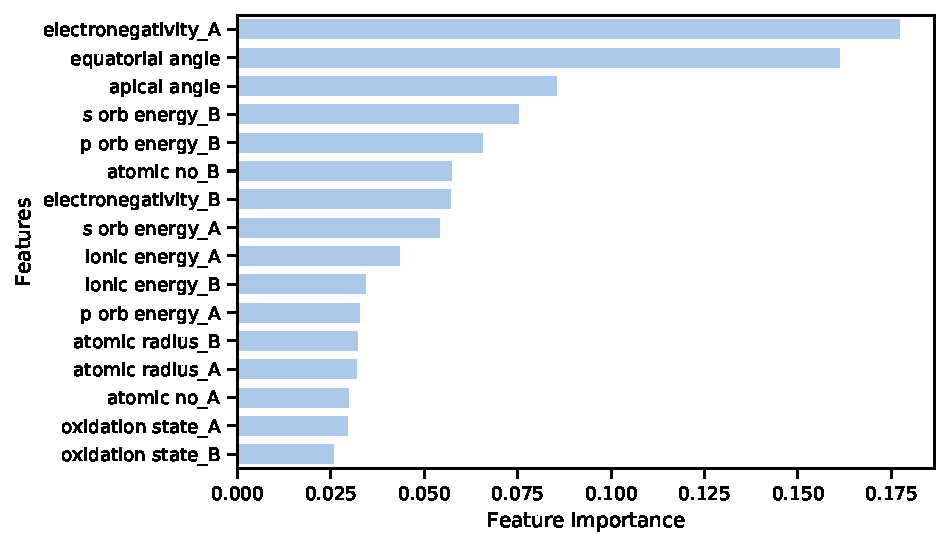
\includegraphics[width=3in]{Figures/feature_ranking_gap.pdf}}%
% \caption{Feature Importance Rankings}
% \label{fig:feature_importance}%
% \end{figure}

%%% VBM and CBM - comparison with photoemission/inverse photoemission exp.
%?????????????
% Note that HSE06 not only corrects band gaps, it also gives band-edge positions, i.e., ionization energies (VBM) and electron affinities (CBM), in much better agreement with experimental data. Determining VBM and CBM positions with respect to vacuum level using periodic supercells requires two separate calculations: one for the bulk material to determine the position of the VBM/CBM with respect to the average electrostatic material which is conventionally set to zero; and another for a slab geometry where average electrostatic potential in the bulk region of the slab is determined with respect potential to the vacuum region. In this case both the thickness of the material and vacuum region have to be large enough to ensure convergence. In Table~\ref{X} of the supplemental material we list the VBM and CBM positions with respect to vacuum of some of the perovskite materials for which experimental data is available.  We see that HSE06 significantly improves the agreement with experimental data compared to DFT-GGA.